

%%%%%%%%%%%%%%%%%%%%%%%%%%%%%%%%%%%55%%
\begin{frame} [plain]
    \frametitle{}
    \Background[1] 
    \begin{center}
    {\huge 第6讲:量子算法(2)    }
    \end{center}  
    \addtocounter{framenumber}{-1}   
\end{frame}
%%%%%%%%%%%%%%%%%%%%%%%%%%%%%%%%%%

\section{1.量子傅里叶变换}

\begin{frame}
    \frametitle{傅里叶变换}
    \begin{itemize}
        \Item 傅里叶变换是科学研究中非常有用的一种数学工具
        \Item 数理机理:找到一组正交完全集,比如$\{e^{ia\omega x}\}$,则任意函数$f(x)$可以在这个集上展开
        \[ f(x)=(\frac{a}{2\pi})^{1/2}\sum_\omega F(\omega) e^{ia\omega x} = (\frac{a}{2\pi}) ^{1/2}\int_{-\infty}^{+\infty} F(\omega) e^{ia\omega x} d\omega\]
        $F(\omega)$为展开(投影)系数:
        \[F(\omega)=\int_{-\infty}^{+\infty}  (e^{ia\omega x}) ^* f(x) dx = \int_{-\infty}^{+\infty}  e^{-ia\omega x} f(x) dx \]
    \end{itemize}
\end{frame}

\begin{frame}
    \frametitle{}
    \begin{itemize}
        \Item 核心应用:把一个非常难解的问题,变换到另一个空间从而成为容易求解,求解后再变换回现有空间,问题得解\\
    \end{itemize}
    \begin{center}
        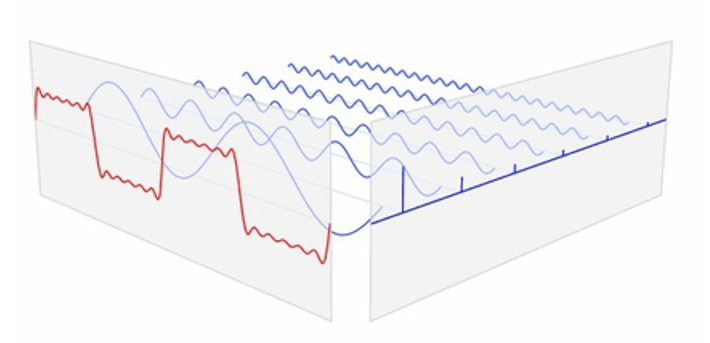
\includegraphics[width=0.7\textwidth]{figs/36.png}
    \end{center}
\end{frame}

\begin{frame}
    \frametitle{}
    {\Bullet} 式中,$a$是伸缩系数,
    $\hspace{1em}$ 通常取$a=1$ \\
    $\hspace{1em}$ 量子力学中,取$a=\dfrac{1}{\hbar}$, 有 
    \[ \Psi(x) = \frac{1}{\sqrt{2\pi \hbar}} \int_{-\infty}^{+\infty} c(p_x) e^{\frac{i}{\hbar}p_x x} dp_x\]
    $\hspace{1em}$ 基矢变换时,取$a=\frac{2\pi}{N}$ \\
    \[ \rs{j} = \frac{1}{\sqrt{N}} \sum_{k=0} ^{N-1} e^{i \frac{2\pi}{N} jk} \rs{k}\]
    $\hspace{1em}$ 不失一般性,可写成 \[ \boxed{\hat{F} \rs{j} = \frac{1}{\sqrt{N}} \sum_{k=0} ^{N-1} e^{i \frac{2\pi}{N} jk} \rs{k}}\]
\end{frame}

\section{2. 傅里叶变换的求和式}

\begin{frame}
    \frametitle{}
    对于一般的态函数,分别在基$\{ \rs{j}\}$和 $\{ \rs{k}\}$ 上展开
    \[\rs{\Psi} =\sum_{j=0} ^{N-1} x_j \rs{j}; \qquad \rs{\Psi} =\sum_{k=0} ^{N-1} y_k \rs{k}\]
    \[\begin{aligned}
        \rs{\Psi} &=\sum_{j=0} ^{N-1} x_j \rs{j} \\
        &=\sum_{j=0} ^{N-1} x_j \frac{1}{\sqrt{N}} \sum_{k=0} ^{N-1} e^{i \frac{2\pi}{N} jk} \rs{k} \\
        &=\sum_{k=0} ^{N-1} \left[\sum_{j=0} ^{N-1} x_j \frac{1}{\sqrt{N}}  e^{i \frac{2\pi}{N} jk} \right]\rs{k} 
    \end{aligned}\]
    \[ \to \qquad y_k = \sum_{j=0} ^{N-1} x_j \frac{1}{\sqrt{N}}  e^{i \frac{2\pi}{N} jk} \qquad \qquad \qquad \qquad\]
\end{frame}

\begin{frame}
    \frametitle{振幅变换公式}
    \[\boxed{y_k = \frac{1}{\sqrt{N}} \sum_{j=0} ^{N-1} x_j  e^{i \frac{2\pi}{N} jk} } \] \vspace{2em}

    $x_j, y_k$分别是 $\rs{\Psi}$ 在基$\{ \rs{j}\}$, $\{ \rs{k}\}$上的展开系数,也称为振幅。 
\end{frame}

\begin{frame}
    \frametitle{}
    \例[已知双量子比特有如下展开式,请展开系数的傅里叶变换形式]
    {\[\rs{\Psi} = a_{00}\rs{00}+ a_{01}\rs{01}+ a_{10}\rs{10}+ a_{11}\rs{11}\]}
    \解~ 在振幅变换公式中,取 N=4, $y_k =  \frac{1}{\sqrt{4}}\sum_{j=0} ^{3} x_j  e^{i \frac{2\pi}{4} jk}$
    \[\begin{aligned}
        y_{00} &=\frac{1}{\sqrt{4}}\sum_{j=0} ^{3} x_j   e^{i \frac{2\pi}{4} j\times 0} = \frac{1}{2}(a_{00}+a_{01}+ a_{10}+ a_{11}) \\
        y_{01} &=\frac{1}{\sqrt{4}} \sum_{j=0} ^{3} x_j  e^{i \frac{2\pi}{4} j\times 1} = \frac{1}{2}(a_{00}+e^{i \frac{\pi}{2}}a_{01}+  e^{i \frac{2\pi}{2}}a_{10}+ e^{i \frac{3\pi}{2}}a_{11}) \\
        y_{10} &=\frac{1}{\sqrt{4}} \sum_{j=0} ^{3} x_j  e^{i \frac{2\pi}{4} j\times 2} = \frac{1}{2}(a_{00}+e^{i \pi}a_{01}+  e^{i 2\pi}a_{10}+  e^{i 3\pi}a_{11}) \\
        y_{11} &=\frac{1}{\sqrt{4}}\sum_{j=0} ^{3} x_j   e^{i \frac{2\pi}{4} j\times 3} = \frac{1}{2}(a_{00}+e^{i \frac{3\pi}{2}}a_{01}+  e^{i \frac{6\pi}{2}}a_{10}+  e^{i \frac{9\pi}{2}}a_{11}) 
    \end{aligned}\]
\end{frame}

\begin{frame}
    \frametitle{小结}
    {\Bullet} 变换后的振幅,差别体现在相位上!\\
    {\Bullet} 量子傅里叶变换可用来做相位估算\\
    {\Bullet} 相位估算是许多量子算法的基础 \\
\end{frame}

\section{3.傅里叶变换的乘积式}

\begin{frame}
    \frametitle{二进制表示}
    考虑傅里叶变换公式的求和形式,可以改写成为:
     \[ \hat{F} \rs{j} = \frac{1}{\sqrt{N}} \sum_{k=0} ^{N-1} e^{i \frac{2\pi}{N} jk} \rs{k} = \frac{1}{\sqrt{N}} \sum_{k=0} ^{N-1} e^{2\pi i  \frac{j}{N} k} \rs{k}\]
    {\Bullet} 注意到 $N=2^n $, $j \le N $ ,式中的$\rs{j}, \dfrac{j}{N}$ 可以写成二进制形式:\\
    $\hspace{1em}$ 设 $ j=\sum\limits_{l=1} ^n j_l 2^{n-l} $; $\quad \frac{j}{N} \approx \sum\limits_{i=1} ^m j_i \frac{1}{2^{i}} $,(m为精度,通常用m=n)
    \begin{itemize}
        \item $\rs{j}= \rs{j_1 j_2 \cdots j_l \cdots j_{n}}$ 
        \item $\dfrac{j}{N} \approx 0. j_{1} j_{2}\cdots j_{i} \cdots j_{m} $ 
    \end{itemize}
\end{frame}

\begin{frame}
    \frametitle{}
    \例[~令 j=9,N=16,m=3 (精度为小数点后三位),写出$\rs{j}$和$\dfrac{j}{N}$的二进制形式] {}
    \解~ $N=16=2^4$,有n=4
    \[j=\sum\limits_{l=1} ^n j_l 2^{n-l} = \sum\limits_{l=1} ^4 j_l 2^{4-l} = 1\times 2^3 + 0\times 2^2 + 0\times 2^1 + 1\times 2^0 \qquad \] 
    \begin{itemize}
        \item $\rs{j}= \rs{9}=\Myitem{t1}{red}{\rs{8+1}}=\Myitem{t2}{red}{\rs{1001}}$ 
    \end{itemize}
    \[\frac{j}{N} = \frac{9}{16} = \Myitem{t3}{red}{\frac{8}{16}+ \frac{1}{16}} = 1\times\frac{1}{2^1} + 0\times\frac{1}{2^2}+ 0\times\frac{1}{2^3} + 0\times\frac{1}{2^4} =\Myitem{t4}{red}{0.1001}\]
    \begin{itemize}
        \item $\dfrac{j}{N} \approx \sum\limits_{i=1} ^m j_i \dfrac{1}{2^{i}} = \sum\limits_{i=1} ^3 j_i \dfrac{1}{2^{i}} = 1\times\dfrac{1}{2^1} + 0\times\dfrac{1}{2^2}+ 0\times\dfrac{1}{2^3} =0.100$
    \end{itemize}
\end{frame}

\begin{frame}
    \frametitle{乘积式}
    傅里叶变换公式的二进制求和形式:
    \[ \hat{F} \rs{j} = \frac{1}{\sqrt{N}} \sum_{k=0} ^{N-1} e^{2\pi i  \frac{j}{N} k} \rs{k}\]
    \[ \hat{F} \rs{j_1j_2\cdots j_n} = \frac{1}{\sqrt{N}} \sum_{k=0} ^{N-1} e^{2\pi i  0.j_1j_2\cdots j_n k} \rs{k}\]
    可以写成如下乘积形式:
    \[\boxed{\hat{F} \rs{j_1j_2\cdots j_n}=\frac{\left[ \rs{0}+ e^{2\pi i 0.j_n} \rs{1} \right]\left[ \rs{0}+ e^{2\pi i 0. j_{n-1}j_n} \rs{1} \right]\cdots \left[ \rs{0}+ e^{2\pi i 0. j_1 j_2 \cdots j_n} \rs{1} \right] }{\sqrt{2}^n }
    }\]
\end{frame}

\begin{frame}
    \frametitle{}
    把$\rs{j}=\rs{j_1 j_2 \cdots j_n} =\rs{00\cdots0}$代入验证:\\
    求和式
    \[ \hat{F} \rs{0} = \frac{1}{\sqrt{N}} \sum_{k=0} ^{N-1} e^{2\pi i \frac{0}{N} k} \rs{k} = \frac{1}{\sqrt{2}^n} \sum_{k=0} ^{N-1} \rs{k}
    \] 
    乘积式
    \[\begin{aligned} 
    \hat{F} \rs{00\cdots 0}
    &=\frac{\left[ \rs{0}+ e^{2\pi i 0.j_n} \rs{1} \right]\left[ \rs{0}+ e^{2\pi i 0. j_{n-1}j_n} \rs{1} \right]\cdots \left[ \rs{0}+ e^{2\pi i 0. j_1 j_2 \cdots j_n} \rs{1} \right] }{\sqrt{2}^n }\\
    &=\frac{\left[ \rs{0}+ e^{2\pi i 0.0} \rs{1} \right]\left[ \rs{0}+ e^{2\pi i 0.00} \rs{1} \right]\cdots \left[ \rs{0}+ e^{2\pi i 0.00 \cdots 0} \rs{1} \right] }{\sqrt{2}^n }\\
    &=\frac{\left[ \rs{0}+  \rs{1} \right]\left[ \rs{0}+  \rs{1} \right]\cdots \left[ \rs{0}+ \rs{1} \right] }{\sqrt{2}^n } \\
    &=\frac{\left[ \rs{00\cdots 0 }+ \rs{00\cdots 1 } +\cdots + \rs{11\cdots 1 } \right] }{\sqrt{2}^n } =\frac{1}{\sqrt{2}^n} \sum_{k=0} ^{N-1} \rs{k} 
    \end{aligned}\]
\end{frame}


\begin{frame}
    \frametitle{等价性证明}
    \begin{itemize}
        \item $k=k_1 2^{n-1}+k_2 2^{n-2}+\cdots+ k_n 2^{0} = \sum_{l=1} ^ n k_l 2^{n-l} $
      \end{itemize} 
    \[\begin{aligned} 
    \rs{j}&= \frac{1}{\sqrt{2^n}}\sum_{k=0} ^{2^n -1} e^{2\pi i j\frac{k}{\color{red}{N}}} \rs{k} \\
    &= \frac{1}{\sqrt{2^n}} \sum_{k_{1}=0} ^{1} \cdots \sum_{k_{n}=0} ^{1} \exp(2\pi i \frac{j}{\color{red}{2^n}}\Myitem{t10}{red}{\sum_{l=1} ^ n k_l 2^{n-l} }) \rs{k_1 k_2 \cdots k_n} \\
    &= \frac{1}{\sqrt{2^n}} \sum_{k_{1}=0} ^{1} \cdots \sum_{k_{n}=0} ^{1} \exp(2\pi i j \Myitem{t2}{red}{\sum_{l=1} ^ n k_l 2^{-l} }) \rs{k_1 k_2 \cdots k_n} \\
    &= \frac{1}{\sqrt{2^n}} \sum_{k_{l}=0} ^{1} \otimes_{l=1} ^n \Myitem{t3}{red}{e^{2\pi i j k_l 2^{-l} }} \rs{k_l} 
    \end{aligned}\]
\end{frame}

\begin{frame}
    \frametitle{}
    \[\begin{aligned} 
    &= \frac{1}{\sqrt{2^n}} \otimes_{l=1} ^n \sum_{k_{l}=0} ^{1} {e^{2\pi i j {\color{red}{k_l}} 2^{-l} }} \rs{k_l} \\
    &= \frac{1}{\sqrt{2^n}} \otimes_{l=1} ^n \left[\rs{0} + e^{2\pi i \color{red}{j 2^{-l}} } \rs{1}\right] \\
    &= \frac{1}{\sqrt{2^n}} \otimes_{l=1} ^n \left[\rs{0} + e^{2\pi i {\color{red}\frac{j}{2^{l}}}} \rs{1}\right] \\
    &= \frac{\left[\rs{0} + e^{2\pi i 0. j_n} \rs{1} \right] \left[\rs{0} + e^{2\pi i 0. j_{n-1} j_n} \rs{1} \right] \cdots \left[\rs{0} + e^{2\pi i 0. j_1 j_2 \cdots j_n} \rs{1} \right] } {\sqrt{2^n}}\\
    \end{aligned}\]
    证毕!\\

    \Tips~ 最后一步,不断地除以2取余,依次得到$j_n, j_{n-1}, \cdots, j_1$, \\
    比如 9/2 余1($j_4$), 4/2 余0($j_3$), 2/2 余0($j_2$), 1/2 余1($j_1$), $9/16=0.1001$  \\  
    又如 8/2 余0($j_4$), 4/2 余0($j_3$), 2/2 余0($j_2$), 1/2 余1($j_1$), $8/16=0.1000$  \\    
\end{frame}

\section{4.傅里叶变换量子线路}

\begin{frame}
    \frametitle{量子线路}
    \begin{center}
        \begin{center}
            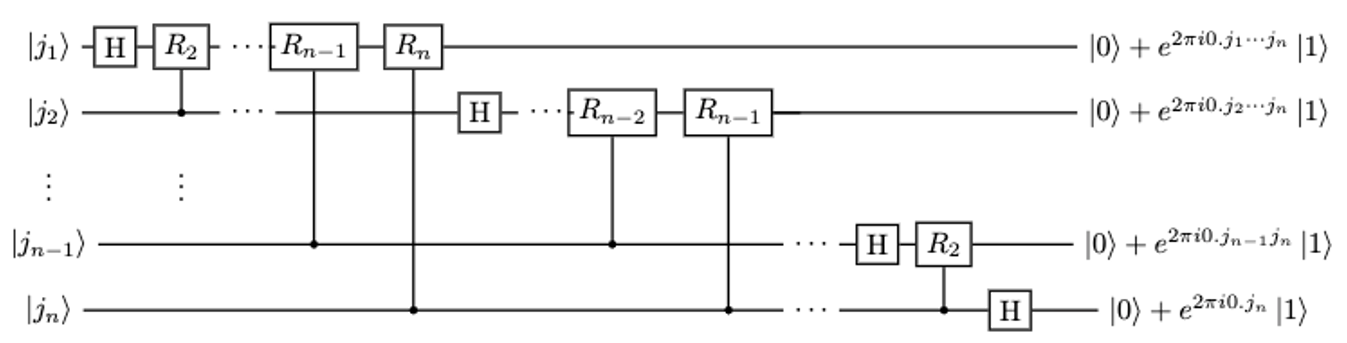
\includegraphics[width=1.0\textwidth]{figs/37.png}
        \end{center}
    \end{center}  
    {\Bullet}~注意:  \\
    \begin{itemize}
        \item 基于乘积式,可设计出如上量子线路
        \item 图中末尾没有给出交换门。
        \item 图中没有给出归一化因子$1/\sqrt{2}$
    \end{itemize}
\end{frame}

\begin{frame}
    \frametitle{推导}
    \begin{center}
        \begin{center}
            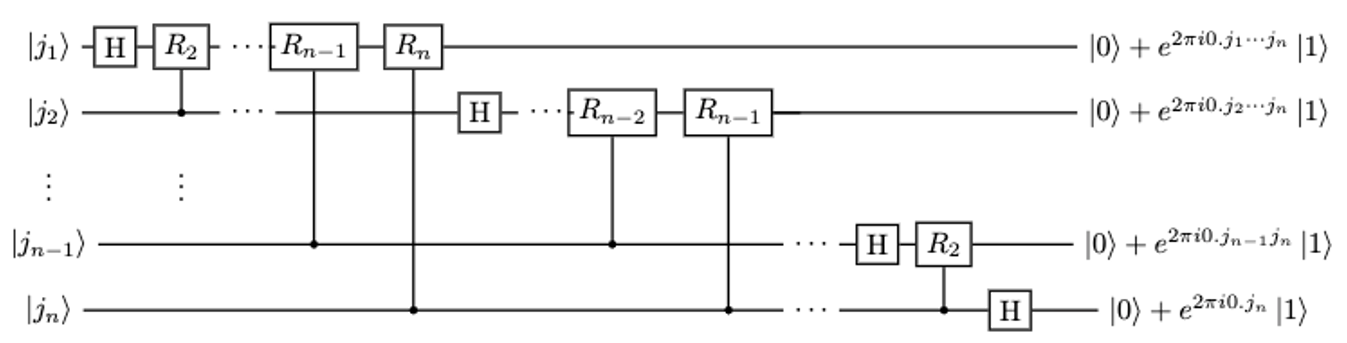
\includegraphics[width=0.9\textwidth]{figs/37.png}
        \end{center}
    \end{center}  
    {\Bullet}~第一个量子位过H门:  \\
    \begin{itemize}
        \item $H\rs{0} \rs{j_2\cdots j_n} = \Pstate \rs{j_2\cdots j_n}= \frac{1}{\sqrt{2}}(\rs{0}+e^{2\pi i 0.j_1}\rs{1}) \rs{j_2\cdots j_n}$
        \item $H\rs{1} \rs{j_2\cdots j_n} = \Mstate \rs{j_2\cdots j_n}= \frac{1}{\sqrt{2}}(\rs{0}+e^{2\pi i 0.j_1}\rs{1}) \rs{j_2\cdots j_n}$
    \end{itemize}
\end{frame}

\begin{frame}
    \frametitle{}
    \begin{center}
        \begin{center}
            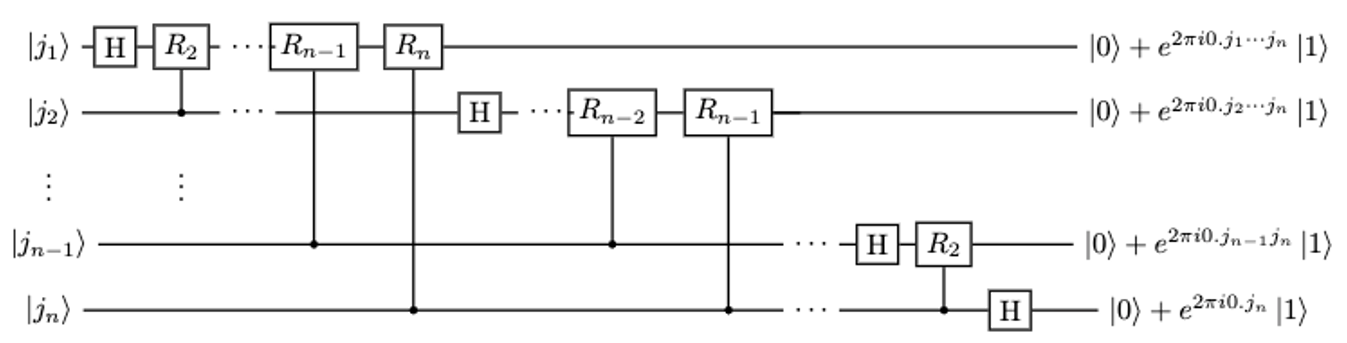
\includegraphics[width=0.9\textwidth]{figs/37.png}
        \end{center}
    \end{center}  
    第一个量子位过受控$R_2$门, ($R_2\equiv e^{i\pi/2}= e^{2\pi i /2^2} $)  \\ \vspace{0.3em}
    \begin{itemize}
        \item $j_2=0, \quad R_2 \frac{1}{\sqrt{2}}(\rs{0}+e^{2\pi i 0.j_1 j_2}\rs{1}) \rs{j_2\cdots j_n}$
        \item $j_2=1, \quad R_2 \frac{1}{\sqrt{2}}(\rs{0}+e^{2\pi i 0.j_1 j_2}\rs{1}) \rs{j_2\cdots j_n}$
    \end{itemize}
\end{frame}


\begin{frame}
    \frametitle{}
    \begin{center}
        \begin{center}
            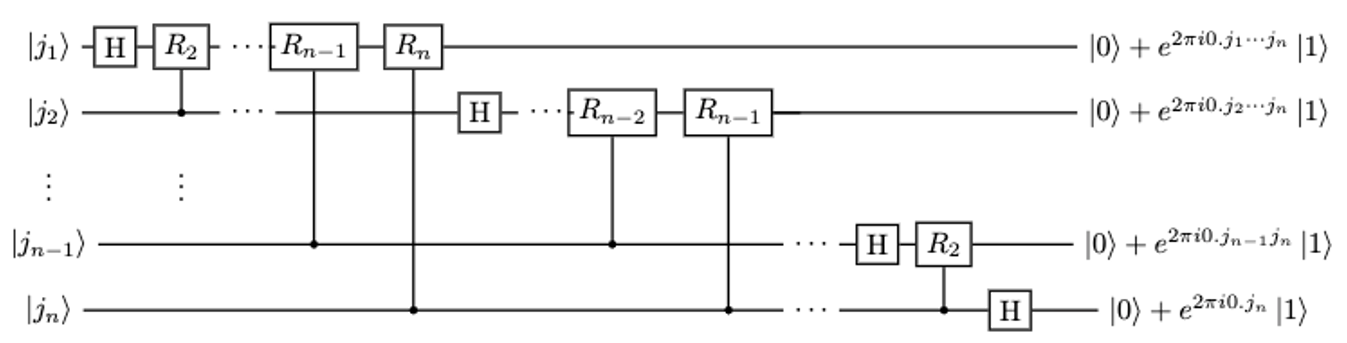
\includegraphics[width=0.9\textwidth]{figs/37.png}
        \end{center}
    \end{center}  
    第一个量子位依次过受控$R_3, R_4, \cdots, R_n$ 门  \\ \vspace{0.3em}
    \begin{itemize}
        \item  $\frac{1}{\sqrt{2}}(\rs{0}+e^{2\pi i 0.j_1 j_2\cdots j_n }\rs{1}) \rs{j_2\cdots j_n}$
    \end{itemize}
\end{frame}

\begin{frame}
    \frametitle{}
    \begin{center}
        \begin{center}
            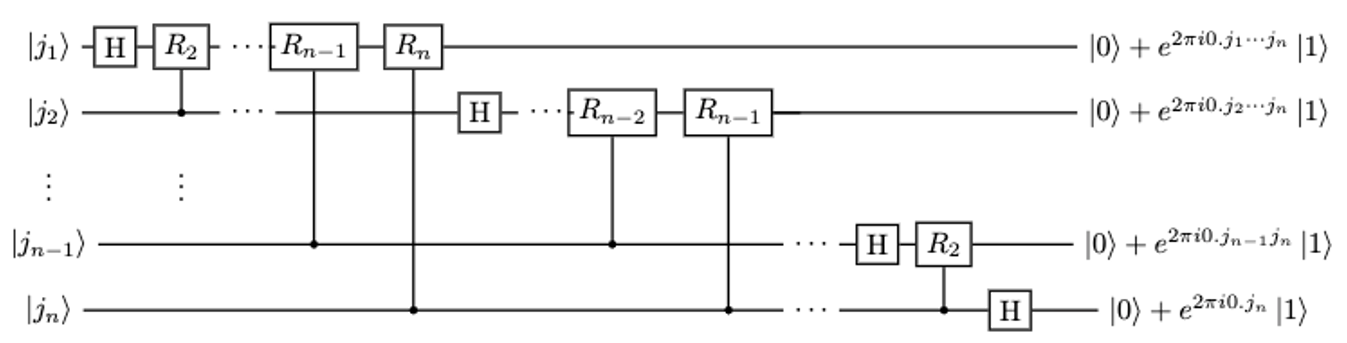
\includegraphics[width=0.9\textwidth]{figs/37.png}
        \end{center}
    \end{center}  
    {\Bullet} 第二个量子位依次过 H门,  \\ \vspace{0.3em}
    \begin{itemize}
        \item  $\frac{1}{\sqrt{2}}(\rs{0}+e^{2\pi i 0.j_1 j_2\cdots j_n }\rs{1}) \frac{1}{\sqrt{2}}(\rs{0}+e^{2\pi i 0.j_2}\rs{1})\rs{j_3\cdots j_n}$
    \end{itemize}
\end{frame}

\begin{frame}
    \frametitle{}
    \begin{center}
        \begin{center}
            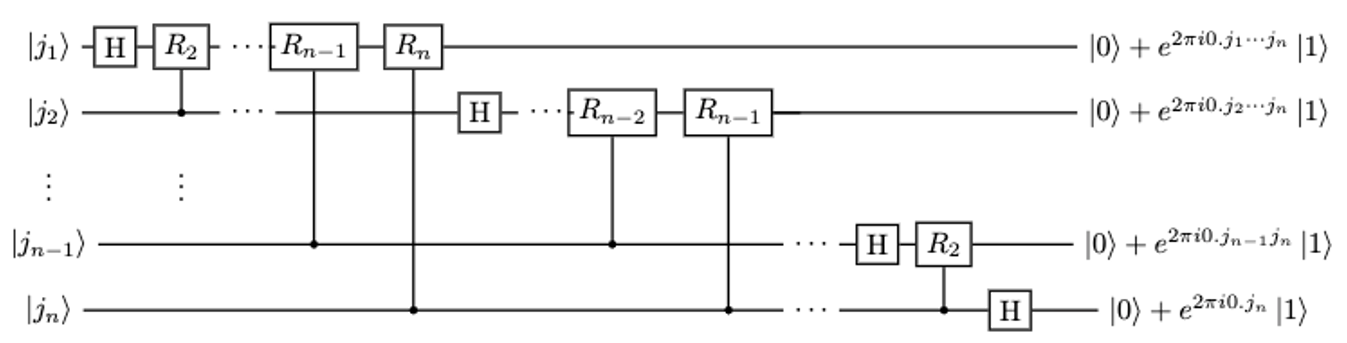
\includegraphics[width=0.9\textwidth]{figs/37.png}
        \end{center}
    \end{center}  
    第二个量子位依次过受控$R_2, R_3, R_4, \cdots, R_{n-1}$ 门  \\ \vspace{0.3em}
    \begin{itemize}
        \item  $\frac{1}{\sqrt{2}}(\rs{0}+e^{2\pi i 0.j_1 j_2\cdots j_n }\rs{1}) \frac{1}{\sqrt{2}}(\rs{0}+e^{2\pi i 0.j_2 j_3\cdots j_{n}}\rs{1})\rs{j_3\cdots j_n}$
    \end{itemize}
\end{frame}

\begin{frame}
    \frametitle{}
    \begin{center}
        \begin{center}
            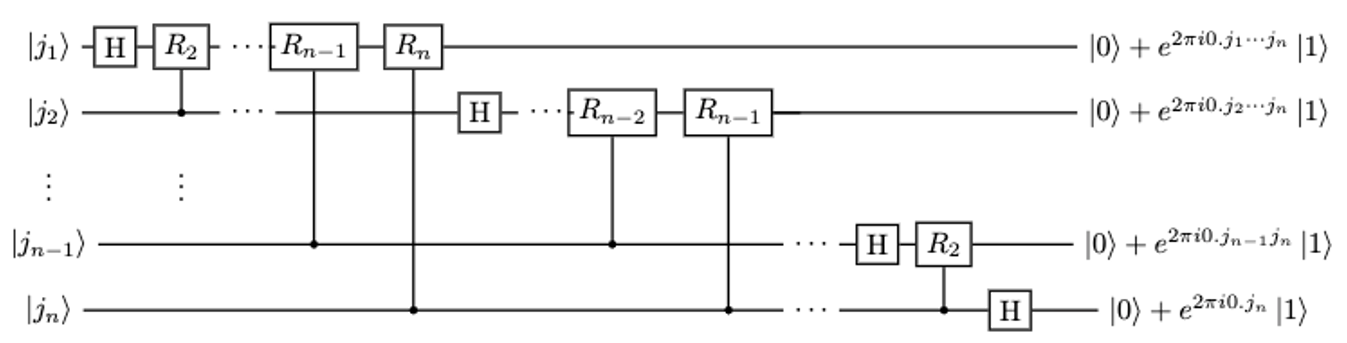
\includegraphics[width=0.9\textwidth]{figs/37.png}
        \end{center}
    \end{center}  
    {\Bullet} 其余各量子位依次类推, 系统的状态变为 \\ \vspace{0.3em}
    \begin{itemize}
        \item  $\frac{1}{\sqrt{2}}(\rs{0}+e^{2\pi i 0.j_1 j_2\cdots j_n }\rs{1}) \frac{1}{\sqrt{2}}(\rs{0}+e^{2\pi i 0.j_2j_3\cdots j_{n}}\rs{1})\cdots \frac{1}{\sqrt{2}}(\rs{0}+e^{2\pi i 0.j_{n}}\rs{1})$
    \end{itemize}
\end{frame}

\begin{frame}
    \frametitle{}
    \begin{center}
        \begin{center}
            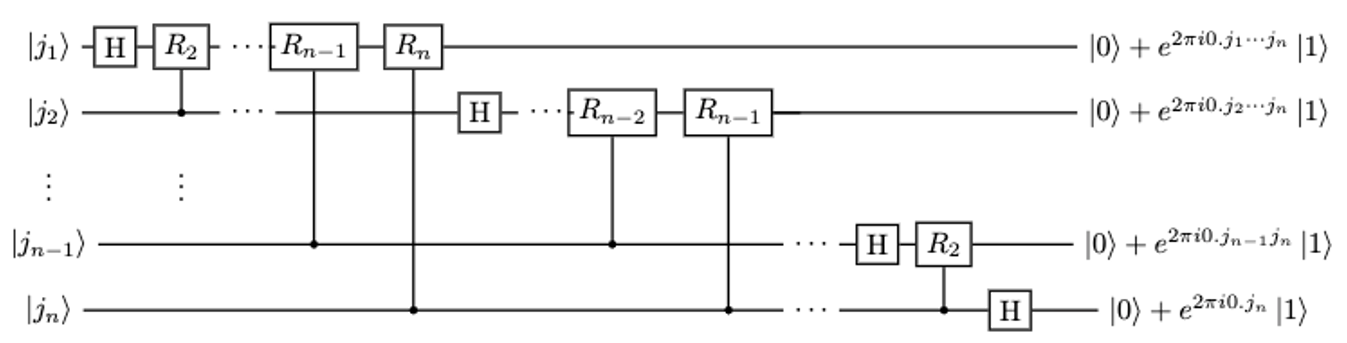
\includegraphics[width=0.9\textwidth]{figs/37.png}
        \end{center}
    \end{center}  
    {\Bullet} 第1与第n位交换,第2与第n-1位交换, $\cdots$ 依次类推, 系统的状态变为 \\ \vspace{0.3em}
    \begin{itemize}
        \item  $\frac{\left[\rs{0} + e^{2\pi i 0. j_n} \rs{1} \right] \left[\rs{0} + e^{2\pi i 0. j_{n-1} j_n} \rs{1} \right] \cdots \left[\rs{0} + e^{2\pi i 0. j_1 j_2 \cdots j_n} \rs{1} \right] } {\sqrt{2^n}}$
    \end{itemize}
    完成!
\end{frame}

\begin{frame}
    \frametitle{复杂度分析}
    {\Bullet} 量子傅里叶变换:第1位使用了n个逻辑门,第2位使用了n-1逻辑门,$\cdots$, 第n位使用了1个逻辑门。共n(n+1)/2个门。交换门n/2. 时间复杂度为$\Theta(n^2)$.\\
    {\Bullet} 经典傅里叶变换:时间复杂度为$\Theta(n 2^n)$.\\
\end{frame}